
\documentclass[11pt]{article} % use larger type; default would be 10pt

%\usepackage{showkeys}

%\newcommand{\ve}{\vfill\eject} 
\newcommand{\ve}{}

%packages
\usepackage{amsmath,amsfonts,amsthm,amssymb,mymath}
\usepackage{fancyhdr,graphicx,lastpage}
\usepackage{enumerate}
\usepackage{graphicx}
\usepackage{graphics}
\usepackage{sidecap}
\usepackage{caption}
\usepackage{floatrow}
%\usepackage{gensymb}
\usepackage{comment}


%setup margins
\topmargin=-0.45in      %
\evensidemargin=0in     %
\oddsidemargin=0in      %
\textwidth=6.5in        %
\textheight=9.0in       %
\headsep=0.25in         %

%Homework specific info
\newcommand{\hmwkTitle}{Homework: 27--43}
\newcommand{\hmwkDueDate}{December 9, 2012}
\newcommand{\hmwkClass}{Math 703}
\newcommand{\hmwkClassTime}{Fall 2012}
\newcommand{\hmwkClassInstructor}{Prof. Girardi}
\newcommand{\hmwkAuthorName}{Blake Farman}

%setup header and footer
\pagestyle{fancy}
\lhead{\hmwkAuthorName, \hmwkClassInstructor, \hmwkClass, \hmwkClassTime}
\chead{}
\rhead{\hmwkTitle}
\lfoot{\hmwkDueDate}
\rfoot{Page\ \thepage\ of\ \pageref{LastPage}}   
\cfoot{}
\renewcommand{\headrulewidth}{0.4pt}                                     
\renewcommand{\footrulewidth}{0.4pt} 
\renewcommand{\headheight}{13.6pt}

%%%%%%%%%%%%%%%%%%%%%%%%%%%%%%%%


\theoremstyle{plain}  % most emphased
\newtheorem{theorem}{Theorem}[section]
\newtheorem{corollary}[theorem]{Corollary}
\newtheorem{lemma}[theorem]{Lemma}
\newtheorem{proposition}[theorem]{Proposition}
\newtheorem{remark}[theorem]{Remark}
\newtheorem*{remarkn}{Remark}
\newtheorem{recall}[theorem]{Recall}
\newtheorem*{factn}{Fact}


\theoremstyle{definition}  %medium emphasised
\newtheorem{definition}[theorem]{Definition}
\newtheorem{notation}[theorem]{Notation}
\newtheorem{gameplan}[theorem]{Game Plan}

\theoremstyle{remark}  %least emphasized 
%\newtheorem{remark}[theorem]{Remark}
%\newtheorem{recall}[theorem]{Recall}
%\newtheorem*{remarkn}{Remark}
\newtheorem{observation}[theorem]{Observation}
\newtheorem{fact}[theorem]{Fact}
\newtheorem{example}[theorem]{Example}
\newtheorem*{question}{Question}
\newtheorem{remarkplain}[theorem]{\textnormal{Remark}}
\newtheorem{notationplain}[theorem]{\textnormal{Notation}}



%\renewcommand{\theequation}{\arabic{section}.\arabic{equation}}

 

%%%%%%%%%%%%%%%%%%%%%%%%%%%%%%%

%%%%%%%%%%%%%%%


\newenvironment{mglist}
{\begin{list}{}{%
\setlength{\leftmargin}{40pt}
\setlength{\rightmargin}{0pt}
\setlength{\itemindent}{0pt}
\setlength{\itemsep}{4pt}
\setlength{\labelsep}{10pt}
\setlength{\labelwidth}{25pt}
}}
{\end{list}}

\newenvironment{zmglist}             % more condensed 
{\begin{list}{}{%
\setlength{\leftmargin}{40pt}
\setlength{\rightmargin}{0pt}
\setlength{\itemindent}{0pt}
%%%%%
\setlength{\itemsep}{0pt}
\setlength{\topsep}{1pt}
\setlength{\parskip}{0pt}
%%%%%%%%
\setlength{\labelsep}{10pt}
\setlength{\labelwidth}{25pt}
}}
{\end{list}}

%%%%%%%%%%%%%%%

%New Commands
 
\newcommand{\ep}{\epsilon}
\newcommand{\e}{\epsilon}
\newcommand{\de}{\delta}
\renewcommand{\phi}{\varphi}

\newcommand{\hsp}[1]{\hskip #1 pt}
\newcommand{\vsp}[1]{\vskip #1 pt}

\newcommand{\dd}{\, d}

\newcommand{\lav}{\left\vert}
\newcommand{\rav}{\right\vert}
\newcommand{\lnm}{\left\Vert}
\newcommand{\rnm}{\right\Vert}
\newcommand{\lp}{\left(}
\newcommand{\rp}{\right)}
\newcommand{\lc}{\left\{}
\newcommand{\rc}{\right\}}

\renewcommand{\Re}{\textrm{Re\,}} 
\renewcommand{\Im}{\textrm{Im\,}}



%%%%%%%%%%%%%%%%%%%%%%%%%%%%%%%%%%%%%%%


\begin{document}

\baselineskip 17 pt 

%%%%%%%%%%%%%%     HW 27  %%%%%%%

% \vsp{5}\noindent\hrulefill

\begin{center}
\textbf{\Large{Homework 27}}
\end{center}

 
\noindent\framebox{
\parbox[t][1.9in]{6.35in}%
{\vsp{5}\noindent
Define $f\colon\C\to\C$ and $u,v\colon\R^2\to\R$ by   
\begin{align*} 
f(z)~&:=~ \sqrt{ \lav xy\rav~}  
\hsp{20}\textrm{where}\hsp{5} x:= \Re z \quad,\quad y:= \Im z 
\\
u(x,y)~&=~ \Re f(x+iy) 
\\
v(x,y)~&=~ \Im f(x+iy) ~.
\end{align*}
Show that 
\begin{zmglist} 
\item[1.] $u$ and $v$ satisfies the Cauchy Riemann equations 
at $(x,y)=(0,0)$ 
\item[2.] $f$ is not differentiable at $z=0$. 
\end{zmglist}
}}

\vsp{8} 

\begin{proof} 
  \begin{enumerate}
  \item
    First observe that $f$ is real-valued, so if we write $f = u + iv$, we have $v \equiv 0$ and $v_x(0,0) = v_y(0,0) = 0$.
    %To show that $f$ satisfies the Cauchy-Riemann equations, we show that the partials of $u$ at $z = 0$ are both zero.
    Now note that when $h \neq 0$ we have
    \begin{align*}
      \frac{u(h,0) - u(0,0)}{h} &= \frac{\sqrt{\abs{0 \cdot h}} - \sqrt{\abs{0 \cdot 0}}}{h} = 0 & \text{and}&& \frac{u(0,h) - u(0,0)}{h} &= \frac{\sqrt{\abs{0\cdot h}} - \sqrt{\abs{0 \cdot 0}}}{h} = 0.
    \end{align*}
    By the definition of the partials for $u$ we have
    \begin{align*}
      u_x(0,0) &= \lim_{h \rightarrow 0} \frac{u(h,0) - u(0,0)}{h} = 0 & \text{and}&& u_y(0,0) & = \lim_{h \rightarrow 0} \frac{u(0,h) - u(0,0)}{h} = 0,
    \end{align*}
    whence $u_x(0,0) = 0 = v_y(0,0)$ and $u_y(0,0) = 0 = -v_x(0,0)$.
    Therefore the Cauchy-Riemann equations are satisfied at $z = 0$.
  \item
    Let $h = 1/n + i/n$.
    Observe that $f(h) = \sqrt{\abs{(1/n^2)}} = 1/n$.
    By the definition of the derivative we have 
    \begin{align*}
      f^\prime(0) = \lim_{n \rightarrow \infty} \frac{f(h) - f(0)}{h} = \lim_{n \rightarrow \infty} \frac{1/n}{1/n(1 + i)} = \lim_{n \rightarrow \infty} \frac{1}{1 + i} = \frac{1 - i}{2} \neq 0.
    \end{align*}
    Therefore $f^\prime(0)$ does not exist, and $f$ is not differentiable at $z = 0$.
  \end{enumerate}
\end{proof}

%%%%%%%%%%%%%%     HW 28  %%%%%%%

% \vsp{5}\noindent\hrulefill
\ve
\begin{center}
\textbf{\Large{Homework 28}}
\end{center}

 
\noindent\framebox{
\parbox[t][1.5in]{6.35in}%
{\vsp{5}\noindent
Let $G$ be the unit disk in $\C$, i.e. 
\begin{equation*} 
G ~=~ B_1(0) ~=~ 
 \lc z\in\C \colon \lav z\rav < 1 \rc. 
\end{equation*}  
Let $f\in H(G)$. 
\begin{zmglist} 
\item[1.] 
Show that if $\Re f$ is constant on $G$  
then $f$ is constant of $G$. 
\item[2.]
Show that if $e^f$ is constant on $G$  
then $f$ is constant of $G$. 
\end{zmglist}
}}

\vsp{8}

\begin{proof}
  \begin{enumerate}
  \item
    For some $u \colon \R^2 \rightarrow \R$ and $v \colon \R^2 \rightarrow \R$ we may write $f = u + iv$ and note that since $u$ is constant, $u_x \equiv 0$ and $u_y \equiv 0$ on $G$.
    %Moreover, since $f$ is holomorphic on $G$, $f$ satisfies the Cauchy-Riemann equations and so $0 \equiv  u_x = v_y$ and $0 \equiv u_y = -v_x$.
    Hence $f' = u_x - iu_y \equiv 0$, and thus all subsequent derivatives are also identically zero on $G$.
    
    Since $f$ is holomorphic on $G$, $f$ is analytic on $G$ and admits a $C^\infty$ power series expansion on an open disc of radius $r < 1$ about $0$,
    $f(x) = \sum_{n=0}^\infty c_n z^n.$
    By the argument above, for every $k \geq 1$ we have %$f^{(k)}(z) \equiv 0$ and the $k^{th}$ derivative is given by the series
    $$0 \equiv f^{(k)}(z) = \sum_{n=k}^\infty c_n(n)(n-1)\ldots(n- k + 1)z^{n - k}.$$
    Evaluating at $z = 0$ we obtain $f^{(k)}(0) = c_k(n)(n-1)\ldots(n - k + 1) = 0$.
    Hence for all $k \geq 1$, $c_k = 0$ and thus $f(z) = c_0$ on $B_r(0)$.
    Since 0 is an accumulation point of $G$, it now follows from the Identity Theorem that $f$ is constant on $G$.
  \item
    For some $z_0 \in \C$ we have $e^f(z) = z_0$.
    Differentiating, we have $f'(z)e^{f(z)} = 0.$
    Since for all $z \in G$, $e^{f(z)} \neq 0$, we have $f'(z) = 0$.
    By the same argument as above, $f$ must be constant on $G$.
  \end{enumerate}
\end{proof}
%%%%%%%%%%%%%%     HW 29  %%%%%%%

% \vsp{5}\noindent\hrulefill
\ve
\begin{center}
\textbf{\Large{Homework 29}}
\end{center}

\noindent\framebox{
\parbox[t][1.7in]{6.35in}%
{\vsp{5}\noindent
Let $G$ be an open subset of $\C$ and $f\in H(G)$. 
Define 
\begin{align*} 
G^* ~&:=~ \lc z\in \C \colon \overline{z} \in G \rc 
\\
f^* (z)~ &:=~ \overline{f(\overline{z})} 
\hsp{20}\textrm{for}\hsp{5} z\in G^*~. 
\end{align*} 
Note   (i.e., you need not show) that $G^*$ is open in $\C$.
\begin{zmglist} 
\item[1.] 
Show that $f^*\in H(G^*)$. 
\item[2.] 
Express $\left( f^*\right)^\prime$ in terms of $f^\prime$. 
\end{zmglist} 
}}

\vsp{8}

\begin{proof}
  Let $\varepsilon > 0$ be given and fix some $z_0 \in G^{\ast}$.
  Since $f$ is holomorphic on $G$ and $\overline{z_0} \in G$, there exists some $\delta > 0$ such that for all $z \in B_\delta(z_0)$
  $$\abs{\frac{f(\overline{z}) - f(\overline{z_0})}{\overline{z} - \overline{z_0}} - f^\prime(\overline{z_0})} < \varepsilon$$
  holds since $\abs{\overline{z} - \overline{z_0}} = ((z - z_0)(\overline{z} - \overline{z_0}))^{\frac{1}{2}} = \abs{z - z_0}< \delta$.
  Now observe similarly that
  \begin{eqnarray*}
    \abs{\frac{f^\ast(z) - f^\ast(z_0)}{z - z_0} - \overline{f^\prime(\overline{z_0})}}
    &=& \abs{\frac{\overline{f(\overline{z})} - \overline{f(\overline{z_0})}}{z - z_0} - \overline{f^\prime(\overline{z_0})}}\\
    &=&\left(\left(\frac{f(\overline{z}) - f(\overline{z_0})}{\overline{z} - \overline{z_0}} - f^\prime(\overline{z_0})\right)\left(\frac{\overline{f(\overline{z})} - \overline{f(\overline{z_0})}}{z - z_0} - \overline{f^\prime(\overline{z_0}})\right)\right)^{\frac{1}{2}}\\
    &=& \abs{\frac{f(\overline{z}) - f(\overline{z_0})}{\overline{z} - \overline{z_0}} - f^\prime(\overline{z_0})} < \varepsilon.\\
  \end{eqnarray*}
  Therefore $f^\ast$ is holomorphic with derivative $\overline{f^\prime}$
\end{proof}

%%%%%%%%%%%%%%     HW  30  %%%%%%%

% \vsp{5}\noindent\hrulefill
\ve
\begin{center}
\textbf{\Large{Homework 30}}
\end{center}

 
\noindent\framebox{
\parbox[t][0.8in]{6.35in}%
{\vsp{5}\noindent
Problem Source: Quals 2004.    
\newline 
Let $G$ be an open connected subset of $\C$. \newline
Let $f\in H(G)$ be s.t.\ 
there is a constant $K\in\R$  with 
$\lav f(z) \rav = K$ for each $z\in G$. \newline
Show that $f$ is constant of $G$. 
}}

\vsp{8}

\begin{proof}
  Let $z_0 \in G$ be an interior point.
  Since $f$ is holomorphic on $G$, $f$ is analytic on $G$ and thus there exists a power series expansion, $f(z) = \sum_{n=0}^\infty c_n(z - z_0)^n$, on a ball $B_R(z_0) \subseteq G$, with $R > 0$.
  Hence $\abs{f(z_0)} = \abs{c_0} = K$.
  
  Suppose to the contrary that $f$ is not constant on $B_R(z_0)$.
  Then by the Open Mapping Theorem, $U = f(B_R(z_0))$ is open and for some $r > 0$, we have $B_r(c_0) \subseteq U$.
  Hence there exists some $z \in f^{-1}(B_r(c_0))$ such that $\abs{f(z)} > \abs{c_0} = K$, a contradiction.
  Therefore $f$ is constant on $B_R(z_0)$, which contains an accumulation point of $G$, and $f$ is constant on $G$ by the Identity Theorem.
\end{proof}
%%%%%%%%%%%%%%     HW 31  %%%%%%%

% \vsp{5}\noindent\hrulefill
\ve
\begin{center}
\textbf{\Large{Homework 31}}
\end{center}

 
\noindent\framebox{
\parbox[t][1.2in]{6.35in}%
{\vsp{5}\noindent
Let $\sum_{n=0}^\infty a_n z^n$ have radius of convergence $R$. 
\newline
What is the radius of convergence of 
the following two power series? 
%\begin{equation*} 
%(1)\quad \sum_{n=0}^\infty a_n \, (2z)^n
%\hsp{30}\textrm{and}\hsp{30} 
%%\sum_{n=0}^\infty (a_n)^2 \, z^n
%\end{equation*}
\begin{enumerate} 
\item 
 $\sum_{n=0}^\infty a_n \, (2z)^n$
\item 
$\sum_{n=0}^\infty (a_n)^2 \, z^n$
\end{enumerate}
}}

\vsp{8}

\noindent 
 You may use, without proving,  Lemma~\ref{l:limsup} 
provided you read the proof I provided below.  
But first, read the handout \textit{lim sup and lim inf of sequences}, 
which is posted on our Math 703/704 homepage. 
In particular, note Claims 10 and 12 of this handout. 


\newcommand{\sn}{\{ s_n\}_{n=1}^\infty}
\newcommand{\lsup}{\varlimsup_{n\to\infty} s_n} 
\newcommand{\linf}{\varliminf_{n\to\infty} s_n}

\begin{factn} \ \newline 
Let $\{ s_n \}_{n=1}^\infty$ be a sequence in $\R$.  
Let $\widehat{\R} := \R \cup \lc \pm \infty \rc$. 
\newline
\underline{Claim 10}. 
There exists a subsequence $\lc s_{n_k} \rc_{k=1}^\infty$ of $\sn$  s.t.  
$\lim_{k\to\infty} s_{n_k} ~=~ \lsup \in \widehat{\R}$. 
\newline
Thus,  if $\sn$ is bounded above, 
then it has a subsequence that converges to an element in $\R$. 
\newline
\underline{Claim 12}. 
\begin{equation*}
\lsup ~=~ \sup \lc \lim_{k\to\infty} s_{n_k} \hsp{5} \colon \hsp{5}
 \lc s_{n_k} \rc_{k=1}^\infty 
\textrm{  is a   subsequence of  $\sn$ s.t.\  } 
\  \lim_{k\to\infty} s_{n_k} \in\widehat{\R} \rc  ~.
\end{equation*}
\end{factn}



\begin{lemma}
\label{l:limsup} 
Let $\{ a_n\}_{n=1}^\infty$ be a bounded sequence of nonnegative 
real numbers.  Then 
\begin{equation*}
\varlimsup_{n\to\infty} \lp a_n\rp^2 
~=~ 
\lp \varlimsup_{n\to\infty} a_n \rp^2~. 
\end{equation*}
\end{lemma} 

\begin{proof} 
LTGBG.  Since $\lc a_n \rc_{n=1}^\infty$, 
and thus also  $\lc \lp a_n\rp^2 \rc_{n=1}^\infty$,  
are bounded above,  the 
$\varlimsup_{n\to\infty} a_n$ and 
$\varlimsup_{n\to\infty} \lp a_n\rp^2$ 
are (finite) real numbers.

\noindent
\fbox{$\leq$}.  
By Claim 10,  there is  a subsequence 
 $\lc  \lp a_{n_k} \rp^2 \rc_{k=1}^\infty$  
 of $\lc \lp  a_n\rp^2 \rc_{n=1}^\infty$ such that 
\begingroup
\setlength{\belowdisplayskip}{0pt}%
\setlength{\abovedisplayskip}{0pt}%
\begin{align*}
 \lim_{k\to\infty} \lp a_{n_k}\rp^2 ~&=~ \varlimsup_{n\to\infty}\lp a_n\rp^2~. 
\intertext{Since the $a_n$'s are nonnegative, 
$\varlimsup_{n\to\infty} a_n \geq 0$. Thus}
\lim_{k\to\infty}  a_{n_k} ~&=~ \sqrt{~ \varlimsup_{n\to\infty}\lp a_n\rp^2~}~. 
\end{align*}
\endgroup
So by Claim 12, 
$\sqrt{~ \varlimsup_{n\to\infty}\lp a_n\rp^2~} ~\leq~
 \varlimsup_{n\to\infty} a_n$. 
    

\noindent
\fbox{$\geq$}.  
By Claim 10,  $\exists$ a subsequence 
 $\lc  a_{n_k}  \rc_{k=1}^\infty$  
 of $\lc  a_n\rc_{n=1}^\infty$ such that 
 $\lim_{k\to\infty}  a_{n_k} = \varlimsup_{n\to\infty} a_n$. 
But then 
 $\lim_{k\to\infty} \lp a_{n_k}\rp^2 = \lp \varlimsup_{n\to\infty} a_n\rp^2$. 
So by Claim 12, 
$ \lp \varlimsup_{n\to\infty} a_n \rp^2 \leq 
\varlimsup_{n\to\infty} \lp a_n\rp^2$.  
\end{proof}


\noindent 
Now
go back  to Homework 1 
([K, Chapter 1, Section 11, \#4) and see if you can find an 
easier proof than the proof that 16 of the 17 students gave. 
I tex-ed up the harder proof since this is how most students 
approached the problem. 

\begin{proof}
  \begin{enumerate}
  \item
    Since $\sum_{n=0}^\infty a_nz^n$ converges for $\abs{z} < R$, $\sum_{n=0}^\infty a_n(2z)^n$ converges when $\abs{z} < R/2$.
  \item
    By Lemma 0.1, $$\limsup \left(\abs{a_n}^{1/n}\right)^2 = \left(\limsup \abs{a_n}^{1/n}\right)^2 = \left(\frac{1}{R}\right)^2 = \frac{1}{R^2}.$$
    Hence the radius of convergence is $R^2$.
  \end{enumerate}
\end{proof}

%%%%%%%%%%%%%%     HW 32  %%%%%%%

\vfill\eject 

% \vsp{5}\noindent\hrulefill

\begin{center}
\textbf{\Large{Homework 32}}
\end{center}

 
\noindent\framebox{
\parbox[t][0.3in]{6.35in}%
{\vsp{5}\noindent
Prove that 
$\sum_{n=1}^\infty \frac{z^n}{n}$ converges for each $z\in\C$ with 
$\lav z\rav =1$ except $z=1$.
}}

\vsp{8}

\noindent 
You may use, without proving, the below \textit{Summation by parts} 
Lemma~\ref{l:sbp}.  

\begin{lemma} 
\label{l:sbp}
Let $\lc a_n \rc_{n=1}^N$ and $\lc b_n \rc_{n=1}^N$ 
be finite sequences of complex numbers.  
Let $B_k = \sum_{l=1}^k b_l$. 
Then for $N>M>1$ 
\begin{equation*} 
\sum_{n=M}^N a_n b_n ~=~ 
a_N B_N ~-~ a_M B_{M-1} ~-~ 
\sum_{n=M}^{N-1} \lp a_{n+1} - a_n \rp B_n ~. 
\end{equation*} 
\end{lemma} 
\begin{proof}[Hint for proof]  
Substitute $b_n = B_n - B_{n-1}$ in the sum on the left. 
\end{proof}

\begin{proof}
  First observe that when $z = 1$, $\sum_{n=1}^\infty \frac{z^n}{n}$ is the Harmonic series, which diverges.
  Assume $\abs{z} = 1$ and $z \neq 1$.
  Take $b_n = z^n$ and $a_n = 1/n$.
  Then we have $B_k = (z^{n+1} - z)/(z - 1)$.
  Using Lemma~\ref{l:sbp} we have for $N > M > 1$ the difference of partial sums
  $$S_N - S_M = \frac{1}{N}{\frac{z^{N+1} - z}{z - 1}} - \frac{1}{M}{\frac{z^{M} - z}{z - 1}} - \sum_{n=M}^{N-1}\left(\frac{1}{n+1} - \frac{1}{n}\right)\frac{z^n - z}{z-1}.$$
  Taking the modulus of both sides and applying the triangle inequality we have
  \begin{equation}\label{32.1}
    \abs{S_N - S_M} \leq \frac{1}{N}\abs{{\frac{z^{N+1} - z}{z - 1}}} + \frac{1}{M}\abs{{\frac{z^{M} - z}{z - 1}}} + \sum_{n=M}^{N-1}\left(\frac{1}{n} - \frac{1}{n+1}\right)\abs{\frac{z^n - z}{z-1}}.
  \end{equation}
  Now we observe that since $\abs{z} = 1$, we have for $n \in \N$
  \begin{equation}\label{32.2}
    \abs{\frac{z^n - z}{z-1}} \leq \frac{\abs{z}^n + \abs{z}}{\abs{z-1}} = \frac{2}{\abs{z-1}}.
  \end{equation}
  Hence by \eqref{32.1} and \eqref{32.2}
  \begin{eqnarray*}
    \abs{S_N - S_M} &\leq& \abs{{\frac{2}{z - 1}}}\left(\frac{1}{N} + \frac{1}{M} + \sum_{n=M}^{N-1}\left(\frac{1}{n} - \frac{1}{n+1}\right)\right)\\
    &=& \abs{{\frac{2}{z - 1}}}\left(\frac{1}{N} + \frac{1}{M} + \frac{1}{M} - \frac{1}{N}\right)\\
    &=& \abs{{\frac{2}{z - 1}}}\left(\frac{2}{M}\right).
  \end{eqnarray*}
  Then as $M$ tends towards $\infty$, the difference in partial sums tends towards zero and the sequence of partial sums is Cauchy.
  Therefore, since $\C$ is complete, $\sum_{n=1}^\infty \frac{z^n}{n}$ converges.
\end{proof}
%%%%%%%%%%%%%%     HW  33  %%%%%%%

% \vsp{5}\noindent\hrulefill
\ve
\begin{center}
\textbf{\Large{Homework 33}}
\end{center}

 
\noindent\framebox{
\parbox[t][1.4in]{6.35in}%
{\vsp{5}\noindent
Let $B_1(0)$ be the open unit disk in $\C$, 
i.e.\ $B_1(0) := \lc z\in\C \colon \lav z \rav < 1 \rc$. 
Show that for $z\in B_1(0)$ 
\begin{equation*} 
\textrm{Log}\, \lp 1-z \rp ~=~ 
\sum_{n=1}^\infty \ -\  \frac{z^n}{n} 
\end{equation*} 
by proving that both sides are holomorphic on $B_1(0)$, 
agree at $z=0$, and have the same derivative on $B_1(0)$. 
}}

\vsp{8}

\noindent 
Hint. Proposition I.4.10 from class notes and also [A, Theorem 3.1.2]. 

\begin{proof}
  Let $f(z) = 1 - z$ and $g = \Log{z}$.
  Observe that $f$ is holomorphic on $B_1(0)$ and $f(B_1(0))$ is the open disc $B_1(1)$.
  Hence $g \circ f$ is holomorphic on on $B_1(0)$.
  Then by Theorem 3.1.2 (Ash) we have 
  $$(g \circ f)^\prime(z) = -\frac{1}{1-z}.$$
  Expanding about $z = 0$ in the usual way, we have the power series
  $$-\frac{1}{1-z} = -\sum_{n=0}^\infty z^n = \sum_{n=0}^\infty -z^n.$$
  Since $\sum_{n=0}^\infty -\frac{z^n}{n}$ converges uniformly on the open unit disc, we have 
  $$\left(\sum_{n=0}^\infty -\frac{z^n}{n}\right)^\prime = \sum_{n=0}^\infty (-\frac{z^n}{n})^\prime = \sum_{n=0}^\infty -\frac{z^n} = -\frac{1}{1-z}.$$
  Since the derivatives of these functions agree, we have that the derivative of their difference has derivative identically zero, and thus the two differ by a constant.
  Namely, 
  $$\Log{1 - z} = \sum_{n=0}^\infty -\frac{z^n}{n} + C.$$
  Taking $z = 0$ we have $0 = \Log{1} = 0 + C.$.
  Therefore $\Log{1 - z} = \sum_{n=0}^\infty -\frac{z^n}{n}$, as desired.
\end{proof}
%%%%%%%%%%%%%%     HW 34  %%%%%%%

% \vsp{5}\noindent\hrulefill
\ve
\begin{center}
\textbf{\Large{Homework 34}}
\end{center}

 
\noindent\framebox{
\parbox[t][0.5in]{6.35in}%
{\vsp{5}\noindent
Let $\gamma$ be the join of the three line segments 
$[1-i, 1+i]$ and $[1+i, -1+i]$ and $[-1+i, -1-i]$. 
Evaluate $\int_\gamma \frac{dz}{z}$ 
by using an appropriate branch of $\log z$. 
}}

\vsp{8} 
\noindent
Hint. See [A, Theorem 3.1.2].

\begin{proof}
  Take $\log(z)$ to be the branch of the logarithm defined on the set $G = \C \setminus \left\{iy \;\middle\vert\; y \in \R,\, y \leq 0\right\}$.
  Then since $\log(z)$ is a primitive for $1/z$ on $G$, the integral is path independent and 
  $$\int_\gamma \frac{dz}{z} = \log(-1 - i) - \log(1 - i) = \log(\sqrt{2}) + i\frac{5\pi}{4} - \log(\sqrt{2}) - i\left(\frac{-\pi}{4}\right) = i\frac{3\pi}{2}.$$
\end{proof}
%%%%%%%%%%%%%%     HW 35  %%%%%%%

% \vsp{5}\noindent\hrulefill
\ve
\begin{center}
\textbf{\Large{Homework 35}}
\end{center}

 
\noindent\framebox{
\parbox[t][1.2in]{6.35in}%
{\vsp{5}\noindent
Compute 
\begin{equation*} 
\int_0^{2\pi}  e^{\cos t} \left[ \cos \lp t+\sin t\rp \right] \, dt 
\hsp{40}\textrm{and}\hsp{40} 
\int_0^{2\pi}  e^{\cos t} \left[ \sin \lp t+\sin t\rp \right] \, dt 
\end{equation*}
by computing $\int_\gamma e^z\, dz$ where $\gamma\colon[0,2\pi]\to\C$ 
is given by $\gamma(t) := e^{it}$. 
}}
\vsp{8}

\begin{proof}
  First observe that the integral of $e^z$ around the closed path $\gamma$ is zero.
  Parameterizing the integral, we obtain
  \begin{eqnarray*}
    \int_\gamma e^z dz &=& i\int_{0}^{2\pi} e^{e^{it}}e^{it}dt\\
    &=& i\int_{0}^{2\pi} e^{\cos(t)}\left(\cos(\sin(t)) + i\sin(\sin(t))\right)\left(\cos(t) + i\sin(t)\right)dt\\
    &=& i\int_{0}^{2\pi} e^{\cos(t)}\left(\cos(\sin(t))\cos(t) - \sin(\sin(t))\sin(t)\right)dt -\\
    & & \int_{0}^{2\pi} e^{\cos(t)}\left(\cos(\sin(t))\sin(t) + \cos(t)\sin(\sin(t))\right)dt\\
    &=& i\int_{0}^{2\pi} e^{\cos(t)}\cos(t + \sin(t))dt - \int_0^{2\pi} e^{\cos(t)}\sin(t + \sin(t))dt\\
    &=& 0 + i0.
  \end{eqnarray*}
  Therefore the value of both integrals is zero.
\end{proof}
%%%%%%%%%%%%%%     HW 36   %%%%%%%

% \vsp{5}\noindent\hrulefill

\vfill\eject 

\begin{center}
\textbf{\Large{Homework 36}}
\end{center}

 
\noindent\framebox{
\parbox[t][1.2in]{6.35in}%
{\vsp{5}\noindent
Let $\alpha\in\C$ with $\lav\alpha\rav\neq 1$. Show that 
\begin{equation*} 
\int_0^{2\pi} 
\frac{d\theta}{1-2\alpha\cos\theta + \alpha^2} 
~=~ 
\frac{i}{\alpha} \int_0^{2\pi} 
\frac{dz}{\lp z-\alpha\rp \, \lp z-\frac{1}{\alpha} \rp} 
\end{equation*} 
where  $\gamma\colon[0,2\pi]\to\C$ 
is given by $\gamma(t) := e^{it}$. 
}}

\vsp{8} 

\begin{proof}
  First observe
  \begin{eqnarray*}
    \frac{1}{1 - 2\alpha\cos(\theta) + \alpha^2} &=& \frac{1}{1 - \alpha\cos(e^{i\theta} + e^{-i\theta})+ \alpha^2}\\
    &=& \frac{1}{(e^{i\theta} - \alpha)(e^{-i\theta} - \alpha)}\\
    &=& \frac{ie^{i\theta}}{-i\alpha(e^{i\theta} - \alpha)(e^{i\theta} - \frac{1}{\alpha})}\\
    &=& \frac{i}{\alpha}\frac{ie^{i\theta}}{(e^{i\theta} - \alpha)(e^{i\theta} - \frac{1}{\alpha})}.\\
  \end{eqnarray*}
  Now, parameterizing the contour integral we have
  \begin{equation*}
    \int_\gamma \frac{dz}{(z - \alpha)(z - \frac{1}{\alpha})} = \int_0^{2\pi} \frac{ie^{i\theta}}{(e^{i\theta} - \alpha)(e^{i\theta} - \frac{1}{\alpha})}.
  \end{equation*}
  Therefore 
  \begin{equation*}
    \int_0^2\pi \frac{1}{1 - 2\alpha\cos(\theta) + \alpha^2}d\theta =   \frac{i}{\alpha}\int_0^{2\pi}\frac{ie^{i\theta}}{(e^{i\theta} - \alpha)(e^{i\theta} - \frac{1}{\alpha})}d\theta = \frac{i}\alpha \int_\gamma \frac{dz}{(z - \alpha)(z - \frac{1}{\alpha})}.
  \end{equation*}
\end{proof}
\noindent 
Hint.  Recall that the function 
$\cos(\cdot) \colon \C \to \C$ 
is defined in   [A, Section 2.3].

%%%%%%%%%%%%%%     HW 37  %%%%%%%

% \vsp{5}\noindent\hrulefill
\ve
\begin{center}
\textbf{\Large{Homework 37}}
\end{center}

 
\noindent\framebox{
\parbox[t][2.0in]{6.35in}%
{\vsp{5}\noindent
Evaluate (without parametrizing the curve $\gamma$, but rather by using 
Cauchy's Integral Theorem) 
\begin{equation*} 
\int_\gamma \frac{dz}{1+z^2} 
\end{equation*} 
for the following $\gamma \colon [0,2\pi]\to\C$. 
\begin{zmglist} 
\item[1.] $\gamma(t) :=  1+ e^{it} $
\item[2.] $\gamma(t) :=  -i + e^{it} $
\item[3.] $\gamma(t) :=  2e^{it} $
\item[4.] $\gamma(t) :=  3i+3e^{it} $
\end{zmglist}
}}

\begin{proof}
  \begin{enumerate}
  \item
    Since $1/(1 + z^2)$ is holomorphic on the set enclosed by $\gamma$, $\int_\gamma \frac{1}{1 + z^2}dz = 0$.
  \item
    Since $-i$ is contained in the set enclosed by $\gamma$, 
    $$\int_\gamma \frac{1}{1 + z^2}dz = 2\pi i(-i - i) = 4\pi.$$
  \item
    Since $\gamma$ encloses both $i$ and $-i$, we separate the integral using the following partial fraction decomposition $1/(1 + z^2) = i/2(z +i) - i/2(z - i)$ to obtain
    $$\int_\gamma \frac{1}{1 + z^2}dz = \frac{i}{2}\left(\int_\gamma \frac{1}{z+i}dz - \int_\gamma \frac{1}{z-i}dz\right) = \frac{i}{2}(2\pi i - 2\pi i) = 0.$$
  \item
    Since $\gamma$ encloses $i$, we have
    $$\int_\gamma \frac{1}{1 + z^2}dz = 2\pi i(2i) = -4\pi.$$
  \end{enumerate}
\end{proof}
%%%%%%%%%%%%%%     HW 38  %%%%%%%

% \vsp{5}\noindent\hrulefill

\ve
\begin{center}
\textbf{\Large{Homework 38}}
\end{center}

 
\noindent\framebox{
\parbox[t][2.0in]{6.35in}%
{\vsp{5}\noindent
Problem Source: Quals 1998. 
 \newline
Fix $a\in\C$ and $r>0$ and let 
\begin{align*} 
B_r(a) ~&:= \lc z\in\C \colon \lav z-a\rav < r\rc
\\
\overline{B_r(a)} ~&:= \lc z\in\C \colon \lav z-a\rav \leq r\rc
\\ 
\partial B_r(a) ~&:= \lc z\in\C \colon \lav z-a\rav = r\rc~.
\end{align*}
Let $G$ be an open set of $\C$ that contains 
 $\overline{B_r(a)}$. 
Let $\lc f_n\rc_{n=1}^\infty$ be a sequence of 
holomorphic functions on $G$ such that 
$\lc f_n\rc_{n=1}^\infty$ converges to the zero function 
uniformly on $\partial B_r(a)$. 
Show that
$\lim_{n\to\infty} f_n(z) = 0$  for each $z\in B_r(a)$.
}}

\vsp{8} 
\noindent 
Hint. Use Cauchy's Integral Formula. 
\vsp{4} 
\noindent 
Remark. 
$\lc f_n\rc_{n=1}^\infty$ converges to the zero function 
uniformly on $\partial B_r(a)$ means that 
\begin{equation*}
\lim_{n\to\infty} \ \sup_{z\in \partial B_r(a)} \lav f_n(z)\rav = 0~.
\end{equation*}

\begin{proof}
  Define the parametrization 
  \begin{align*}
    \gamma \colon [0,2\pi] &\rightarrow \C\\
    \theta &\mapsto a + re^{i\theta}.
  \end{align*}
  Fix some $z_0 \in B_r(a)$.
  By the Cauchy Integral Forumla, we have for each $n \in \N$
  $$f_n(z_0) = \frac{1}{2\pi i}\int_\gamma \frac{f_n(z)}{z - z_0} dz.$$
  Letting $n$ tend to infinity we have by uniform convergence 
  $$\lim_{n \rightarrow \infty} f_n(z_0) = \lim_{n \rightarrow \infty} \frac{1}{2\pi i}\int_\gamma \frac{f_n(z)}{z - z_0} dz = \frac{1}{2\pi i}\int_\gamma \lim_{n \rightarrow \infty}\frac{f_n(z)}{z - z_0} dz = 0.$$
\end{proof}


%%%%%%%%%%%%%%     HW 39  %%%%%%%

% \vsp{5}\noindent\hrulefill

\vfill\eject 

\begin{center}
\textbf{\Large{Homework 39}}
\end{center}

 
\noindent\framebox{
\parbox[t][1.2in]{6.35in}%
{\vsp{5}\noindent
Problem Source: Quals 1995. 
\newline 
Let $f\in H(\C)$ satifsy, 
for some constants $A,B\in\R$ and $k\in\N$, 
\begin{equation*} 
\lav f(z) \rav ~\leq~ A \lav z\rav^k + B 
\end{equation*} 
for each $z\in \C$.  Prove that $f$ is a polynomial. 
}}

\begin{proof}
  Consider the path along the boundary of a ball $B_r(0)$ parametrized by
  \begin{align*}
    \gamma \colon [0,2\pi] &\rightarrow \C\\
    \theta &\mapsto a + re^{i\theta}.
  \end{align*}
  By the Cauchy Estimate, we have
  $$\abs{f^{(m)}(0)} \leq \frac{n!}{r^n} A\abs{z}^k + B.$$
  Letting $r$ tend to infinity, we see that if $m > k$, $f^{(m)}(0) = 0$.
  
  Since $f$ is entire, it has some power series expansion of radius $R$ centered about 0, $f(z) = \sum_{n=0}^\infty c_nz^n$.
  Then for $m > k$, the derivative is given by
  $$f^{(m)}(0) = c_m(n)(n-1)\ldots(n-m+1) = 0.$$
  Hence for $m > k$ we have $c_m = 0$ and thus on $B_R(0)$
  \begin{equation}\label{39.1}
    f(z) = \sum_{n=0}^\infty c_nz^n = \sum_{n=0}^k c_nz^n.
  \end{equation}
  Since $B_R(0)$ contains a limit point of $\C$, we have that \eqref{39.1} holds for all of $\C$ by the Identity Theorem.
\end{proof}
%%%%%%%%%%%%%%     HW 40   %%%%%%%

% \vsp{5}\noindent\hrulefill

\ve
\begin{center}
\textbf{\Large{Homework 40}}
\end{center}

 
\noindent\framebox{
\parbox[t][1.6in]{6.35in}%
{\vsp{5}\noindent
Problem Source: Quals 1995.  

\noindent 
 Let $G$ be an open connected subset of $\C$. 
Let $\lc f_n \rc_{n=1}^\infty$ be a sequence  
from $H(G)$  and $f\colon G \to \C$ be a function 
 satisying 
\begin{gather} 
\label{40-1}\tag{40.1}
\begin{split}
\textrm{for each compact subset $K$ of $G$,}
\phantom{\hsp{100}}
\\
\textrm{the functions 
$\lc f_n\vert_K \rc_{n=1}^\infty$  converge 
uniformly on $K$ to $f\vert_K$~.} 
\end{split}
\end{gather}
Show that   $f\in H(G)$. 
}}

\begin{proof}
  Fix some $a \in G$ and choose $r > 0$ such that $\overline{B_r(a)} \subseteq G$ so that $f_n$ converges uniformly there.
  Since $B_r(a)$ is star-like, for any triangle, $\Delta$, contained inside $B_r(a)$, we have $\int_\Delta f_n(z)dz = 0$.
  Then by uniform convergence, we have 
  $$\lim_{n \rightarrow \infty}\int_\Delta f_n(z)dz = \int_\Delta \lim_{n \rightarrow \infty} f_n(z)dz = \int_\Delta f(z)dz = 0.$$
  Since $\Delta$ was arbitrary, it follows from Morera's Theorem, that $f$ is holomorphic on $B_r(a)$, and thus holomorphic at $a$.
  Since $a$ was arbitrary, $f$ is holomorphic on $G$.
\end{proof}
%%%%%%%%%%%%%%     HW 41  %%%%%%%

% \vsp{5}\noindent\hrulefill

\ve
\begin{center}
\textbf{\Large{Homework 41}}
\end{center}

 
\noindent\framebox{
\parbox[t][1.1in]{6.35in}%
{\vsp{5}\noindent
Problem Source: Quals 2000.  

\noindent 
Let $f$ be an entire function such that, for some $M>0$, 
\begin{equation*} 
\lav f(z) \rav \leq M e^{\Re z} 
\hsp{20}\forall z\in \C~. 
\end{equation*} 
Show that there exists $K\in\C$ such that 
$f(z) = K e^z$. 
}}

\begin{proof}
  Since $e^z$ does not have any zeroes, the function $f(z)/e^z$ is entire.
  Then $$\abs{f(z)/e^z} = \abs{f(z)}e^{\real{z}} \leq Me^{\real{z}}/e^{\real{z}} = M$$ implies, by Liouville's Theorem, that $f/e^z$ is constant.
  Therefore $f(z) = Ke^z$, as desired.
\end{proof}

%%%%%%%%%%%%%%     HW  42  %%%%%%%

% \vsp{5}\noindent\hrulefill

\ve
\begin{center}
\textbf{\Large{Homework 42}}
\end{center}

 
\noindent\framebox{
\parbox[t][0.8in]{6.35in}%
{\vsp{5}\noindent
Problem Source: Quals 1999.  

\noindent
Show that 
\begin{equation*} 
\int_0^\pi e^{\cos\theta} \cos\lp\sin\theta\rp\, d\theta ~=~ \pi~. 
\end{equation*}  
}}

\vsp{8}\noindent 
Hint. Consider $\int_{\gamma} \frac{e^z}{z}\, dz$ where 
$\gamma\colon [0,2\pi]\to\C$ is given by 
$\gamma(\theta) = e^{i\theta}$. 



%%%%%%%%%%%%%%     HW 43  %%%%%%%

% \vsp{5}\noindent\hrulefill

\begin{proof}
  Let $\gamma\colon [0,2\pi]\to\C$ be given by $\gamma(\theta) = e^{i\theta}$, which encloses 0.
  Then we have by the Cauchy Integral Formula
  $$2\pi i = \int_\gamma \frac{e^z}{z}dz = i\int_0^{2\pi} e^{e^{i\theta}}d\theta = i\int_0^{2\pi} e^{\cos(\theta)}(\cos(\sin(\theta)) + i\sin(\sin(\theta)))d\theta$$
  Comparing coefficients, we have 
  $$2\pi  = \int_0^{2\pi} e^{\cos(\theta)}\cos(\sin(\theta))d\theta = 2\int_0^{\pi} e^{\cos(\theta)}(\cos(\sin(\theta))d\theta.$$
  Therefore $\pi = \int_0^{\pi} e^{\cos(\theta)}(\cos(\sin(\theta))d\theta$, as desired.
\end{proof}
\vfill\eject

\begin{center}
\textbf{\Large{Homework 43}}
\end{center}

 
\noindent\framebox{
\parbox[t][1.2in]{6.35in}%
{\vsp{5}\noindent
Problem Source: Quals 1997.  

\noindent 
Let $\gamma^*$ be as in Figure 1 below.  Find 
\begin{equation*} 
\int_\gamma \frac{1+z+z^3}{z(z-1)(z-i)} \, dz ~. 
\end{equation*}
}}

\begin{proof}
  Observe that the poles $i$ and 0 are enclosed by a a single curve the pole 1 is enclosed by two curves.
  All other closed curves do not contain poles and are thus zero.
  Hence the value of the integral is given by
  $$2\pi i \left(\frac{1 + i + i^3}{i(1-i)}\right) + 2\pi i\left(\frac{1 + 0 + 0^3}{(0 - 1)(0 - i)}\right) + 4\pi i \left(\frac{1 + 1 + 1^3}{1(1 - i)}\right) = \pi(1 + i) + 2\pi + 6\pi(i - 1) = -3\pi + i7\pi$$
\end{proof}

\begin{center} 
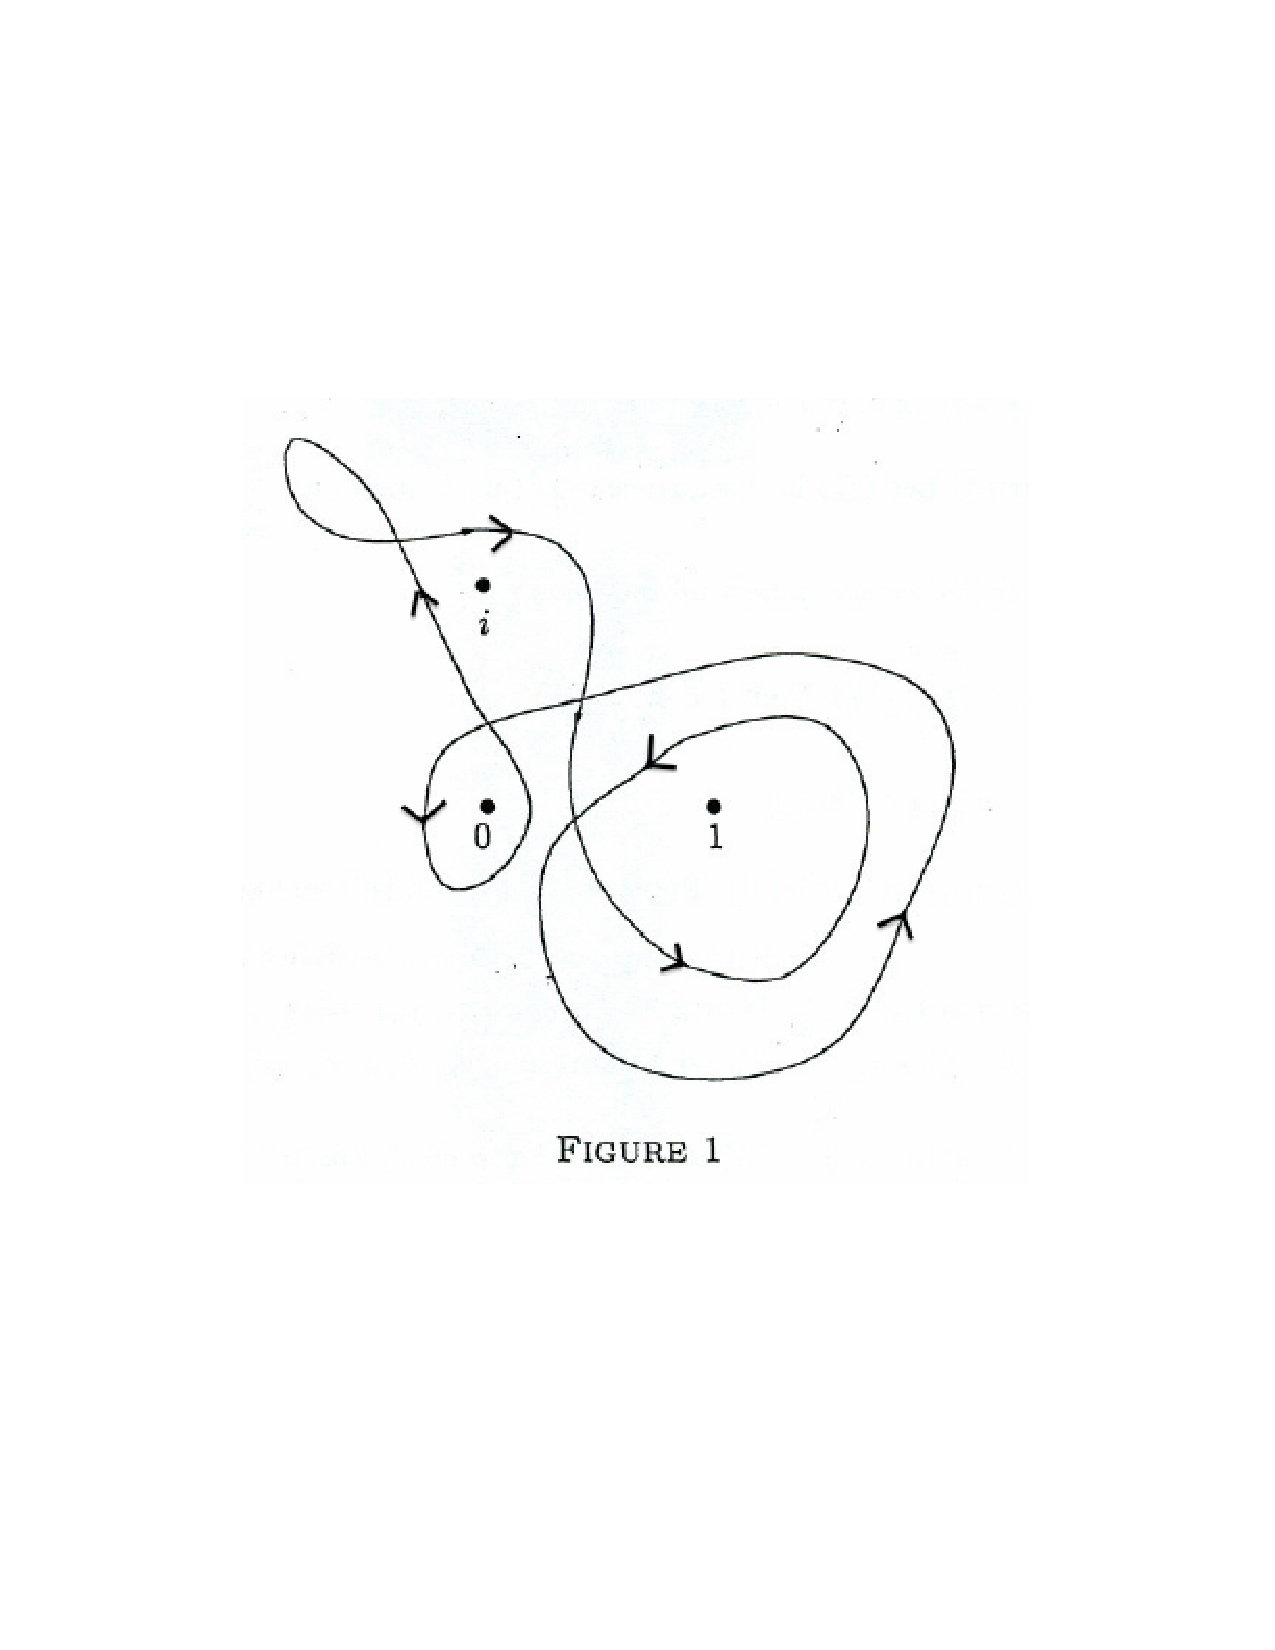
\includegraphics[scale=0.4]{43funkycurve.pdf}
\end{center}
%%%%%%%%%%%%%%    



\end{document}

 
